\section{FSMDriver}\label{sec:3}%
Driving a car can be intuitively divided into several behaviors, and thus provide a straightforward implementation as a finite-state machine model. Such model's configuration parameters can be optimized through a genetic algorithm, and the TORCS/SCR platform provides a standard measure of driver quality, and its sensor/actuator interface enable it to be readily replaced by actual robotic prototypes (or other more advanced models) for further testing. This work proposes to use these ideas for evolving a controller for a car, the FSMDriver, as one more step towards autonomous vehicles.

\newcommand{\state}[1]{\texttt{#1}}%
\newcommand{\SL}{\state{Straight Line}}%
\newcommand{\C}{\state{Curve}}%
\newcommand{\OT}{\state{Out of Track}}%
\newcommand{\St}{\state{Stuck}}%
\newcommand{\AC}{\state{Approaching Curve}}%
\newcommand{\IT}{\state{Inside Track}}%

\subsection{Driving Behaviors}%
A \state{State} in the FSM model considered here defines a racing behavior, deciding the driver's output according to the given sensor input as defined by SCR's API. The FSM implements a transition function that, at every game tick, analyses the input and decides which state is appropriate, triggering a change if necessary. The state then processes the input and defines the proper output.

The next step for implementing the FSM model is defining its states. Intuitively, \state{Driving}~could be a definite solution but it obviously involves several distinct situations which should be divided, simplifying the development.

Considering the testing environment, it is clear that two antagonistic situations that require specific behaviors: \state{Racing}, for situations where the car is within track limits, facing the right direction; and \state{Recovery}, for when the car is outside track limits or facing the right direction, or unable to move.

These can be further divided into two more specific behaviors for implementation:
\begin{description}
	\item[\SL:] for racing straight ahead;
	\item[\C:] for racing through a curve;
	\item[\OT:] for recovering from leaving the track or facing the wrong direction; and
	\item[\St:] for recovering from being unable to move forward.
\end{description}

Each of these states implements its behavior as follows. \SL~ attempts to go as fast as possible parallel to the track axis by accelerating at full throttle, and changing gears according to RPM thresholds. \C~steers towards the direction towards the track sensor with the largest reading (see Figure~\ref{Fig:FSensor}) with 60\% throttle, braking in case it starts to slide in the X axis. \OT~ attempts to return to the track, facing the right direction, adjusting its speed and steering according to its current orientation concerning the track (see Figure~\ref{Fig:Angle}). \St~ tries to get unstuck by using the reverse gear and hard steering.

\begin{figure}[h]
	\centering
	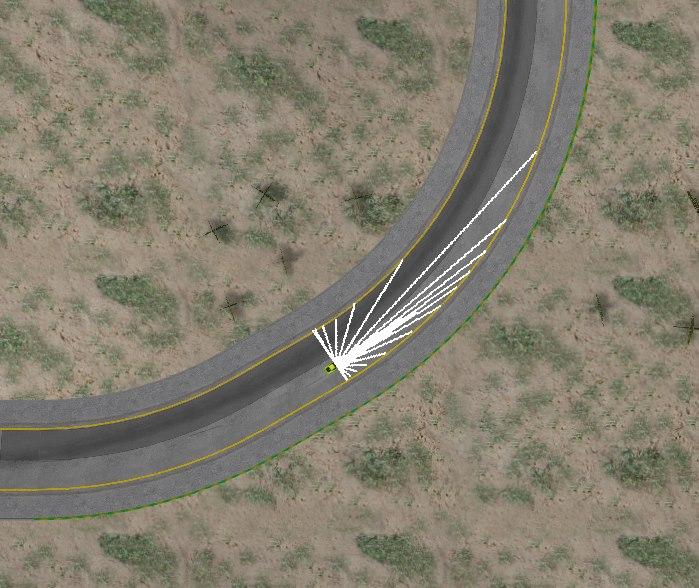
\includegraphics[width=.45\textwidth]{img/FarthestSensor}
	\caption{Sensor input in curve.}
	\label{Fig:FSensor}
\end{figure}

\begin{figure}%[h]
		\centering
		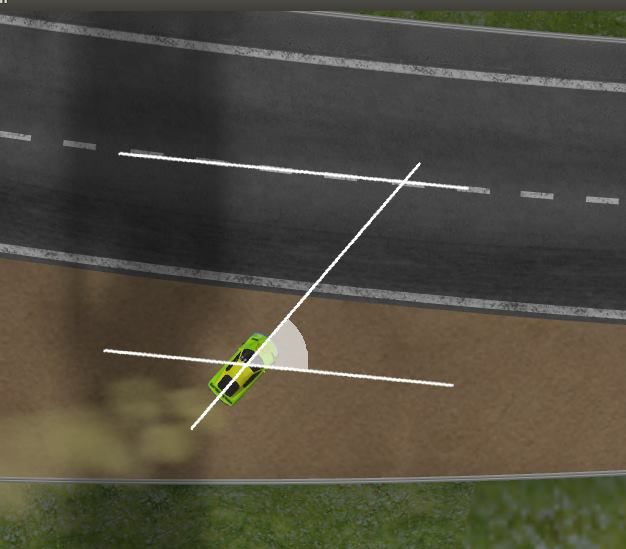
\includegraphics[width=.45\textwidth]{img/ReturnAngle}
		\caption{Angle between car and track axis.}
		\label{Fig:Angle}
\end{figure}

\subsection{FSMDriver5}

Initial tests showed that transitioning from \SL~to \C~was too swift, hampering performance because the car consistently entered curves at such high speeds that the controller was unable to turn and exited the track, so the additional behavior \AC~was implemented. \AC~ positions the driver towards the outside of the incoming curve and tries to race at a speed proportional to the curvature, so less braking would be necessary in \C. Thus, a 5-state FSMDriver (FSMDriver5) model (illustrated in Figure~\ref{Fig:FSM5Diagram}) was ready for testing.

\begin{figure}[h]
	\centering
	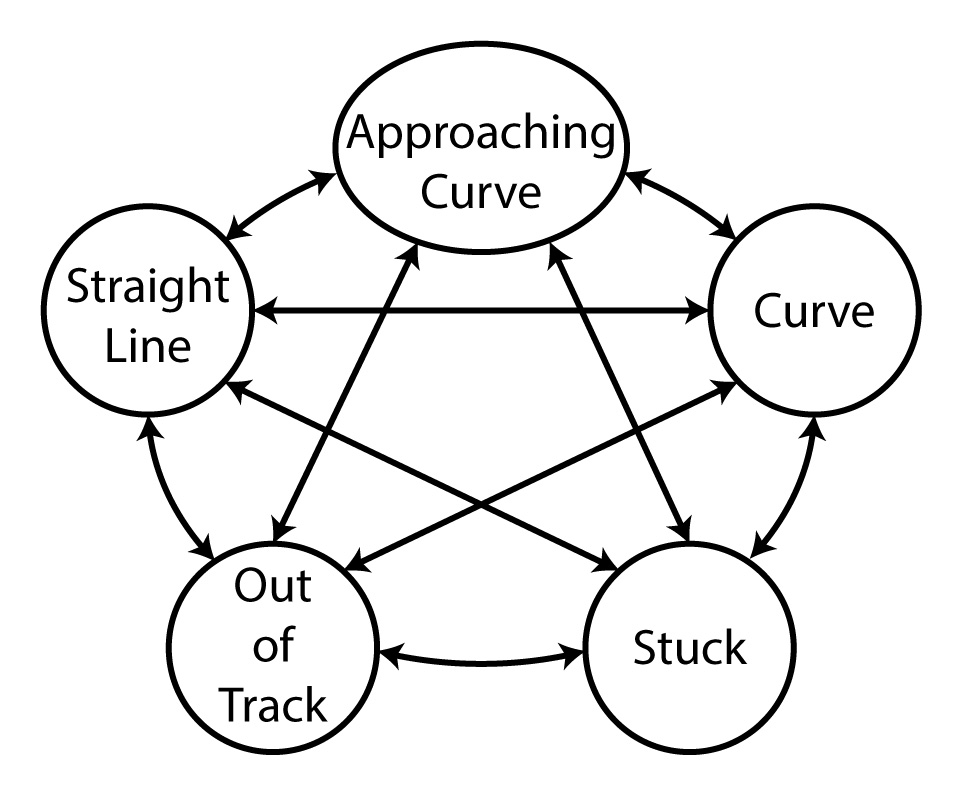
\includegraphics[width=.45\textwidth]{img/FiveStateFSM}
	\caption{FSMDriver5 state diagram.}
	\label{Fig:FSM5Diagram}
\end{figure}

The range sensors were arbitrarily configured at every $10$ degrees from $-90$ to $90$ relative to the car's front axis (that is, a uniform distribution from the left to the right of the car), as illustrated in Figure~\ref{Fig:FSM5Sensors}.

\begin{figure}[h]
	\centering
	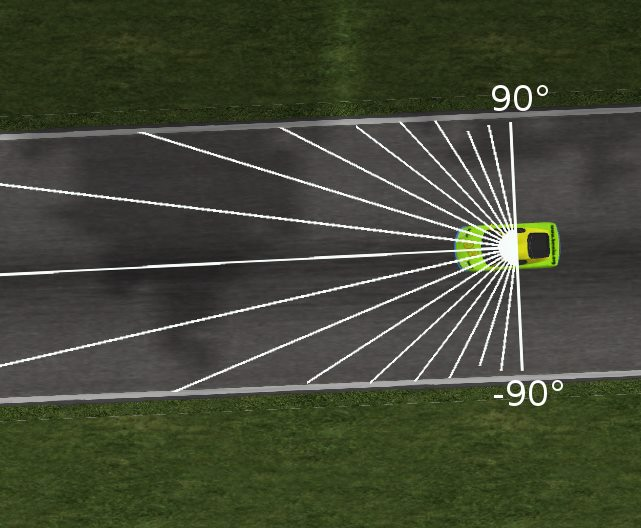
\includegraphics[width=.45\textwidth]{img/FSM5Sensors}
	\caption{FSMDriver5 range finders.}
	\label{Fig:FSM5Sensors}
\end{figure}

Sensor readings provide an idea of location in the track, in this setting, the difference between frontal and lateral sensors is larger when driving in a straight line than in a curve. Thus, the transition function considers the variance of readings from range finders to define the current state of the \state{Racing} behavior, as described in Algorithm~\ref{alg:FSMDriver5}.

\begin{algorithm}[h]%
\caption{FSMDriver5 Transition}%
\label{alg:FSMDriver5}%
\begin{algorithmic}
    \IF{car is stuck}
        \STATE $state \Leftarrow Stuck$
    \ELSE
		\IF{$variance$ is in $StraightLine$ thresholds \AND
		the current state is not $StraightLine$}
			\STATE $state \Leftarrow StraightLine$
		\ELSIF{$variance$ is not in $ApproachingCurve$ thresholds \AND
		current state is not $Curve$}
			\STATE $state \Leftarrow ApproachingCurve$
		\ELSIF{$variance$ is in $ApproachingCurve$ thresholds \AND
		current state is not $ApproachingCurve$}
			\STATE $state \Leftarrow ApproachingCurve$
		\ELSIF{$variance > 0$}
			\STATE $state \Leftarrow Curve$
		\ELSE
			\STATE $state \Leftarrow Out Of Track$
		\ENDIF
	\ENDIF
\end{algorithmic}
\end{algorithm}

The variance is computed as follows: \gnramos{como é calculada?}

Initially, random configurations were set and manually adjusted until an acceptable behavior was achieved, i.e. such a configuration in which a car could successfully complete a race. In the beginning, the \state{Recovery} states (\OT~and \St) were constantly triggered, and therefore were first to be adjusted for improved behavior. Eventually their settings were such that the \state{Racing} behaviors could be focused on. These too were manually and arbitrarily set through trial and error, considering the driver's quantitative performance racing (time and damage) and its qualitative skill (visual analysis of tests).

After several iterations, this model performed better performance than some of the less capable robots available in TORCS,showcasing the FSM model's potential for controlling a car. However, testing also revealed that the transitions between states required were the bottleneck for improved racing. Not only some of the triggers needed a more detailed analysis to avoid eventual erratic behavior, but the sheer number parameters considered for transitioning, each with its triggers (see Figure~\ref{Fig:FSM5Diagram}), and their impact on the model's behavior during a complete race caused the whole model to be thought over.

Analyzing FSMDriver's transitions occurrences within a race, it was clear that the \state{Recovery} behavior had two distinct situations, which were acceptably handled by the current configuration, and that the major issue was frequent triggering between the \state{Racing} states, which inevitably resulted in the car leaving the track and jeopardizing its performance.

\subsection{FSMDriver3}%
To reduce the model's complexity, and considering the intuitive division of behaviors proposed, a new model where the defined \state{Recovery} behaviors were maintained and the \state{Racing} behaviors were joined into a new state called \IT. Figure~\ref{Fig:FSM3Diagram} illustrates this FSMDriver3 model.

\begin{figure}[h]
	\centering
	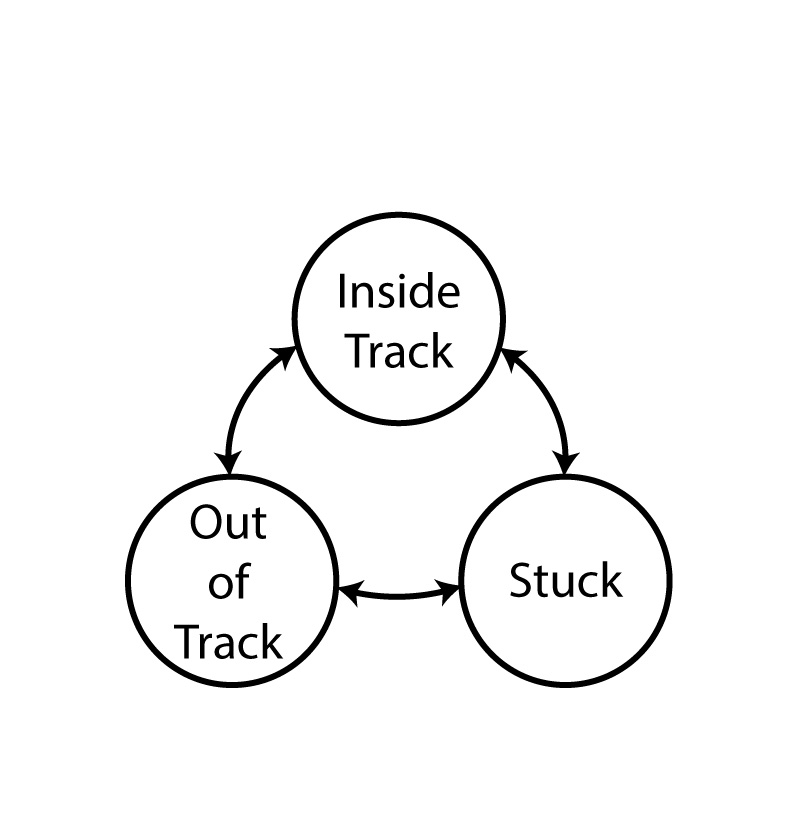
\includegraphics[width=.4\textwidth]{img/ThreeStateFSM}
	\caption{FSMDriver3 state diagram.}
	\label{Fig:FSM3Diagram}
\end{figure}

\IT~implements a very straightforward idea, get to an arbitrary target speed towards the largest open space inside track limits. The target speed is proportional to the largest sensor reading, and braking is activated if the current speed is greater than the target. Gear changing works based on RPM threshold as before. Overall, this implementation works for straight lines as well as curves.

In order to have more detailed information on track segment straight ahead, which will guide the movement, the range finders are concentrated in front of the car, as shown in Figure~\ref{Fig:FSM3Sensors}, contrasting with FSMDriver5's equidistant distribution.

\begin{figure}[h]
	\centering
	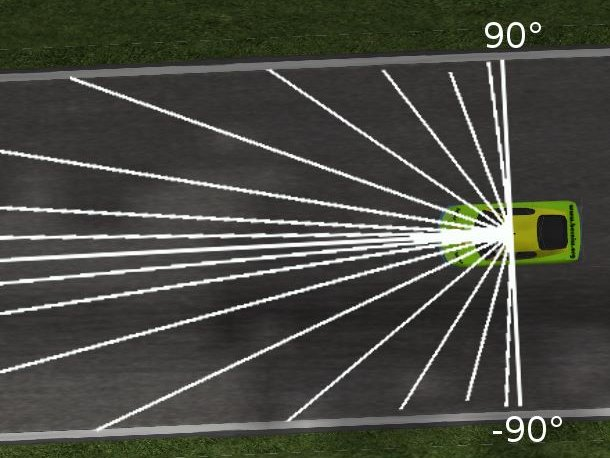
\includegraphics[width=.45\textwidth]{img/FSM3Sensors}
	\caption{FSMDriver3 range finders.}
	\label{Fig:FSM3Sensors}
\end{figure}

The transition function can then be reimplemented in a simpler fashion, as shown in Algorithm~\ref{alg:FSMDriver3}:

\begin{algorithm}[h]%
\caption{FSMDriver3 Transition}%
\label{alg:FSMDriver3}%
\begin{algorithmic}
    \IF{car is stuck}
        \STATE $state \Leftarrow Stuck$
    \ELSE
        \IF{car is within track limits}
            \STATE $state \Leftarrow Inside Track$
        \ELSE
            \STATE $state \Leftarrow Outside Track$
        \ENDIF
    \ENDIF
    \IF{the current state is not $state$}
        \STATE $Current State \Leftarrow state$
    \ENDIF
\end{algorithmic}
\end{algorithm}

Initially, configurations resembling FSMDriver5's parameters were set and manually adjusted until a behavior similar to the original driver was achieved. As expected, this process was quicker than for FSMDriver5 and soon a configuration better than some robots was available.

With the finished models\footnote{Code available at \url{https://github.com/bruno147/fsmdriver}}, the issue at hand became to set the models' parameter to such values as to maximize their performance, a large combinatorial problem to which a well known tool was applied.

\subsection{Offline Learning: Evolving Parameters}%
In order to apply a genetic algorithm to the task of evolving the drivers' parameters, a model of the solution must be defined. In this context, a solution is called an individual and was represented by a string of bits, which compose the floating point parameters of the models.

FSMDriver5 has, overall, 22 parameters implemented in states and the transition function. The function considers 4 threshold values defining 2 intervals, one for identifying the variance levels for \SL~ (\texttt{MIN\_STRAIGHTLINE\_VAR} and \texttt{MAX\_STRAIGHTLINE\_VAR} and another for \AC~(\texttt{MIN\_APPROACHING\_CURVE\_VAR} and \texttt{MIN\_APPROACHING\_CURVE\_VAR}). \SL~ also considers 4 threshold values, one for changing gears (\texttt{LOW\_GEAR\_LIMIT}), and 3 for identifying RPM values that indicate when to increase/decrease gear (\texttt{LOW\_RPM}, \texttt{AVERAGE\_RPM}, and \texttt{HIGH\_RPM}).

\AC~has 3 parameters, a desired position \gnramos{em relacao a que?} (\texttt{TARGET\_POS}), a lower speed threshold (\texttt{BASE\_SPEED}) and a maximum steering value (\texttt{MAX\_STEERING}). \OT considers 7 parameters two angle thresholds for returning to the track inter (\texttt{MIN\_RETURN\_ANGLE} and \texttt{MAX\_RETURN\_ANGLE}), 3 speed thresholds for changing gears (\texttt{VELOCITY\_GEAR\_2}, \texttt{VELOCITY\_GEAR\_3}, and \texttt{VELOCITY\_GEAR\_4}), a breaking threshold to avoid skidding (\texttt{MAX\_SKIDDING}) defines the threshold to start breaking to avoid skidding and, finally, a value for defining this decelerating intensity (\texttt{NEGATIVE\_ACCEL\_PERCENT}), defined with the axis speed of car.

\St has 4 parameters, one for defining a starting distance before considering the car stuck (\texttt{MINIMUM\_DISTANCE\_RACED}), one for tracking the speed \texttt{STUCK\_SPEED}, and two for defining game ticks thresholds for actions' duration in order to trigger a transition to this state (\texttt{MAXIMUM\_NUMBER\_OF\_TICKS\_STUCK} and \texttt{MAXIMUM\_NUMBER\_OF\_TICKS\_IN\_SLOW\_SPEED}).

FSMDriver3, on the other hand, has the same 11 for \OT~and \St~ as FSMDriver5, and 6 additional for \IT. There is one for changing gears (\texttt{LOW\_GEAR\_LIMIT}), 3 for identifying RPM values that indicate when to increase/decrease gear (\texttt{LOW\_RPM}, \texttt{AVERAGE\_RPM}, and \texttt{HIGH\_RPM}), one for defining a ratio between car speed and range finder reading for setting the target speed (\texttt{SPEED\_FACTOR}), and a minimal speed value \gnramos{para que?} (\texttt{BASE\_SPEED}).

The GA also requires a fitness function to evaluate the solutions, this work will consider the distance raced, which is also the standard metric for SCR. This means that the GA has to communicate with the test platform, calling  TORCS and simulating races with the drivers, and processing the results. The simulation is run through operating system calls and the results communicated through shared memory\footnote{Code available at \url{https://github.com/bruno147/driver-ga}}.

\subsection{Online Learning: Staying in Track}%
An online learning module was included in FSMDriver3 trying to improve its performance, in an attempt to reduce damage and time loss for racing out of the track. Whenever the driver enters \OT, the speed and location of this occurrence are recorded and used in the \state{Racing} state. If the speed is over an arbitrary value (85 km/h \gnramos{é km/h?}), the model assumes the driver has left the track due to excessive speed and uses this information to slow down the driver in subsequent laps when approaching the recorded places, trying to remain inside the track.

This behavior does not interfere with the breaking actions in the model, but does affect the driver's performance and, thus, with the offline learning process. Though FSMDriver5 can also learn where it leaves the track, the differences in implementation of the \state{Racing} states are such that slowing down before the target places implies on excessive additional complexity.